\section{Results and Discussion}

\subsection{Model Selection and Fine-Tuning (Tasks 1 and 2)}
\textbf{Training behaviour.} Fig.~\ref{fig:train} (left) shows the completion-token loss falling from about 0.2 to below 0.03 within the 152 optimiser steps; the right panel shows validation scores per epoch. For the selected run (v1) validation macro-F1 peaked at epoch~1 (0.481) and then drifted down to 0.436, while accuracy peaked at epoch~2 (0.748) and evidence F1 kept improving until epoch~4 (0.610). With only 8 validation patients and a handful of rare-class examples, macro-F1 moves by several points between epochs, so this selection is noisy. We nevertheless kept the pre-declared rule (best validation macro-F1), which selects epoch~1. The alternative v2, with fully inverse-frequency sampling ($p{=}1$), under-trained the majority classes: its best validation macro-F1 was 0.395 and its first-epoch accuracy only 0.437 with four unparsable outputs, so it was rejected. The 0.5B draft, trained with the same recipe, reached validation macro-F1 0.540 (epoch~3), which we kept for speculative decoding.

\begin{figure*}[t]
\centering
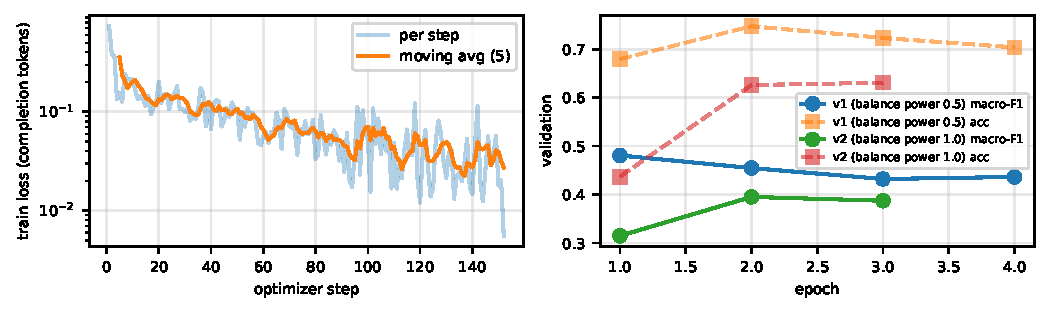
\includegraphics[width=\textwidth]{fig_train.pdf}
\caption{Training loss of the selected 1.5B run (left) and validation macro-F1 / accuracy per epoch for v1 and v2 (right).}
\label{fig:train}
\end{figure*}

\textbf{Before vs.\ after fine-tuning.} On the validation split the base model scores accuracy 0.087, macro-F1 0.095 and evidence F1 0.126 against 0.680/0.481/0.496 after tuning (epoch~1). Table~\ref{tab:main} gives the held-out test results, evaluated once. The zero-shot model rarely follows the required JSON schema (7 invalid outputs) and reaches an accuracy of 0.121; the adapted model reaches 0.723, macro-F1 0.685 and evidence micro-F1 0.559 with no invalid output. The two trivial baselines show what a model must beat: always predicting the training-majority label per criterion type already gives 0.626 accuracy (because 62.6\% of test criteria carry the majority label of their type) but only 0.272 macro-F1, and citing sentence~0 gives evidence F1 0.253. Hence the gain over the majority baseline is modest in accuracy (+0.097) but large in macro-F1 (+0.41) and evidence F1 (+0.31). We did not compute significance tests; with 206 criteria from 8 patients, differences of a few points should not be over-interpreted.

\begin{table}[t]
\caption{Held-out test results (206 criteria, 8 patients), before/after tuning and baselines. Generation: Hugging Face \texttt{generate}, fp16, batch 16, greedy with the model's default repetition penalty of 1.1 (see text).}
\label{tab:main}
\centering\scriptsize
\begin{tabular}{lcccc}\toprule System & Acc & Macro-F1 & Evid. $\mu$-F1 & Invalid\\\midrule
Majority label per type + sentence 0 & 0.626 & 0.272 & 0.253 & 0\\
Qwen2.5-1.5B zero-shot (before) & 0.121 & 0.172 & 0.167 & 7\\
Qwen2.5-1.5B + LoRA (after) & 0.723 & 0.685 & 0.559 & 0\\
\bottomrule\end{tabular}
\end{table}

\textbf{Decoding settings matter.} Qwen's bundled generation configuration sets a repetition penalty of 1.1 that Hugging Face applies even when sampling is disabled. Table~\ref{tab:main} was produced with this default, exactly as in the training-time validation. Our own engine implements plain greedy decoding (no penalty). Re-scoring the same held-out set with our engine (fp16, batch size 1, KV cache, argmax) gives accuracy 0.728, macro-F1 0.708 and evidence micro-F1 0.531 (inclusion 0.853/0.633/0.588; exclusion 0.656/0.484/0.410). Pure greedy is slightly better on accuracy and macro-F1 and worse on evidence F1; we regard the two runs as equivalent within noise and use the engine's decoding in the application.

\textbf{Inclusion vs.\ exclusion and per-class behaviour.} Table~\ref{tab:split} separates the two criterion types and Table~\ref{tab:perclass} lists per-class scores of the Table~\ref{tab:main} model. Inclusion is clearly easier (accuracy 0.840, evidence F1 0.66) than exclusion (0.656, 0.32). The test split contains no \emph{excluded} example (Table~\ref{tab:dist}), so macro-F1 is computed over the five classes that occur. For inclusion, \emph{included} (F1 0.87) and \emph{not enough information} (0.88) are handled well, \emph{not included} reaches F1 0.67 on only 7 examples, and \emph{not applicable} is never found (0 of 3). For exclusion, \emph{not excluded} (F1 0.79) dominates; \emph{not enough information} has recall 0.11 (3 of 28), i.e.\ the model usually asserts that an exclusion criterion does not apply when the note is merely silent, which is precisely the failure mode the task warns about. Fig.~\ref{fig:conf} shows the confusion matrices.

\begin{table}[t]
\caption{Test results separated by criterion type, with evidence precision/recall/F1 (micro).}
\label{tab:split}
\centering\scriptsize
\begin{tabular}{llcccc}\toprule System & Subset & Acc & Macro-F1 & Evid. P/R/F1 & n\\\midrule
Qwen2.5-1.5B zero-shot (before) & inclusion & 0.227 & 0.197 & 0.31/0.45/0.37 & 75\\
Qwen2.5-1.5B zero-shot (before) & exclusion & 0.061 & 0.077 & 0.03/0.25/0.06 & 131\\
Qwen2.5-1.5B + LoRA (after) & inclusion & 0.840 & 0.603 & 0.63/0.69/0.66 & 75\\
Qwen2.5-1.5B + LoRA (after) & exclusion & 0.656 & 0.484 & 0.38/0.28/0.32 & 131\\
\bottomrule\end{tabular}
\end{table}

\begin{table}[t]
\caption{Per-class precision, recall and F1 on the test set for the model of Table~\ref{tab:main}.}
\label{tab:perclass}
\centering\scriptsize
\begin{tabular}{llcccc}\toprule Subset & Class & P & R & F1 & Support\\\midrule
inclusion & included & 0.885 & 0.852 & 0.868 & 27\\
inclusion & not applicable & 0.000 & 0.000 & 0.000 & 3\\
inclusion & not enough information & 0.818 & 0.947 & 0.878 & 38\\
inclusion & not included & 0.800 & 0.571 & 0.667 & 7\\
exclusion & not applicable & 0.467 & 0.583 & 0.519 & 12\\
exclusion & not enough information & 0.231 & 0.107 & 0.146 & 28\\
exclusion & not excluded & 0.745 & 0.835 & 0.788 & 91\\
\bottomrule\end{tabular}
\end{table}

\begin{figure*}[t]
\centering
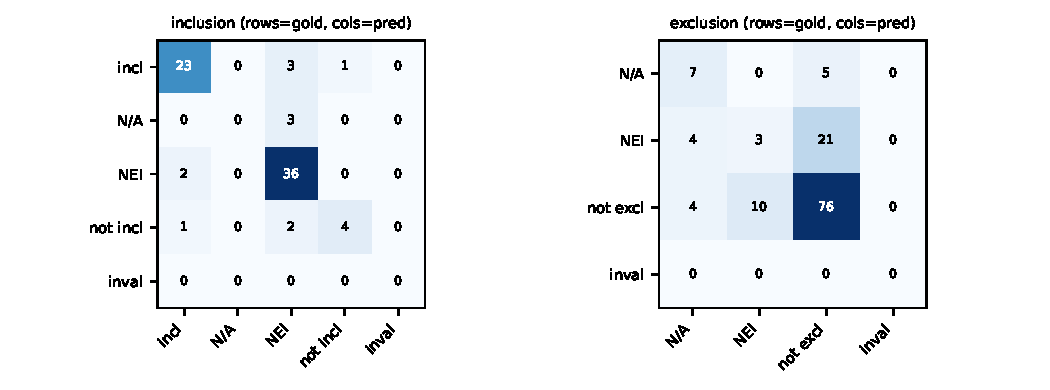
\includegraphics[width=0.85\textwidth]{fig_conf.pdf}
\caption{Test confusion matrices for inclusion and exclusion criteria (NEI = not enough information).}
\label{fig:conf}
\end{figure*}

\subsection{Error Analysis}
The model makes 57 label errors on the 206 test criteria. Table~\ref{tab:errors} lists twelve of them, one per distinct error type. We discuss them with the caveat that we did not trace internal causes; the explanations are hypotheses consistent with the outputs.
\begin{itemize}
\item \emph{Missing information treated as absence (cases 2, 5, 11).} For ``previous axillary surgery'' the gold label is \emph{not enough information} but the model answers \emph{not excluded} without citing any sentence; the application flags such answers as \emph{unsupported}. In case 11 the vague criterion ``Genetic patients'' is labelled \emph{included} with sentence~0 as evidence although the experts found the note uninformative.
\item \emph{Contradictory or hallucinated evidence (1, 7).} In case 1 the model cites sentence~1 to claim an exclusion that the experts judge not met; in case 7 it cites sentence~0 to support \emph{included} where the gold evidence set is empty. Both are fluent but wrong justifications.
\item \emph{Applicability confusion (4, 5, 6, 12).} The model predicts \emph{not applicable} for contraception-related exclusions that experts mark \emph{not excluded} or \emph{not enough information}, and the reverse in cases 6 and 12. Our reading is that \emph{not applicable} depends on patient characteristics (e.g.\ sex) that are expressed only indirectly in the note.
\item \emph{Negated criteria (8).} For ``No medical history of central vena catheterization'' the gold label is \emph{included} but the model says \emph{not included}, a typical negation inversion.
\item \emph{Missed or partial evidence (3, 10).} In case 3 the label is wrong though the right sentence is cited, and in case 10 the model cites sentence~0 whereas the experts used sentences 2 and 3, leading to \emph{not enough information} instead of \emph{included}.
\item \emph{Silent under-prediction (9).} For ``Maintenance hemodialysis after central vena catheterization'' the model predicts \emph{not enough information} and cites nothing, while the experts mark \emph{not included}.
\end{itemize}
Overall, errors cluster around information that is absent or implicit, which suggests that more annotated data or retrieval of related criteria would help more than additional epochs.

\begin{table*}[t]
\caption{Representative test errors, one per distinct error type (NEI = not enough information; ev. = evidence sentence IDs).}
\label{tab:errors}
\centering\scriptsize
\begin{tabular}{p{0.4cm}p{6.5cm}p{2.3cm}p{2.3cm}p{1.4cm}p{1.4cm}}\toprule \# & Criterion (truncated) & Gold & Pred & Gold ev. & Pred ev.\\\midrule
1 & Significant upper limb peripheral arterial disease & not excluded & excluded & [] & [1]\\
2 & Patients with previous axillary surgery & NEI & not excluded & [] & []\\
3 & Less than 18 years of age & not excluded & NEI & [0] & [0]\\
4 & Pregnant women or women of childbearing age who do not have adequate c... & not excluded & not applicable & [0] & []\\
5 & Female subject of child-bearing potential who is not using a medically... & NEI & not applicable & [] & [0]\\
6 & Symptoms that collectively suggest nonstreptococcal T/P (eg, laryngiti... & not applicable & not excluded & [0] & [0]\\
7 & Patients undergoing surgical lower limb revascularisation (suprainguin... & not included & included & [] & [0]\\
8 & No medical history of central vena catheterization. & included & not included & [0] & [0]\\
9 & Maintenance hemodialysis after central vena catheterization. & not included & NEI & [] & []\\
10 & Patients were included if they were diagnosed with Shock, Acute respir... & included & NEI & [2, 3] & [0]\\
11 & Genetic patients & NEI & included & [] & [0]\\
12 & If female, using birth control & not applicable & NEI & [3] & [3]\\
\bottomrule\end{tabular}
\end{table*}

\subsection{KV-Cached Generation (Task 3)}\label{sec:kv}
\textbf{Correctness.} Table~\ref{tab:equiv} compares our cached decoder with the no-cache reference and with Hugging Face \texttt{generate} for nine input/output length combinations (input prompts built from real test prompts, 128/512/1024 tokens; 16/64/128 forced output tokens, no early stopping). Cached and no-cache outputs are identical in all nine cases. Against \texttt{generate} with its default configuration six of nine differ, at positions 11--63; with the repetition penalty set to 1.0 all nine are identical, which shows that the discrepancy comes from the penalty and not from our implementation. In addition, on all 206 real test prompts our engine reproduces plain-greedy \texttt{generate} outputs exactly (206/206). In fp32 our forward pass matches Hugging Face to a maximum logit difference of $8.5\times10^{-5}$ with identical argmax at every position; in fp16 the corresponding difference on the same prompt is 0.088 and not all argmaxes agree, which is the expected size of half-precision rounding noise.

\begin{table}[t]
\caption{Cached decoding versus references (fp16, greedy). ``HF default'' includes Qwen's repetition penalty 1.1; ``HF pure'' sets it to 1.0.}
\label{tab:equiv}
\centering\scriptsize
\begin{tabular}{rrccc}\toprule In & Out & = no-cache & = HF default & = HF pure\\\midrule
128 & 16 & yes & yes & yes\\
128 & 64 & yes & no (@24) & yes\\
128 & 128 & yes & no (@24) & yes\\
512 & 16 & yes & no (@11) & yes\\
512 & 64 & yes & no (@11) & yes\\
512 & 128 & yes & no (@11) & yes\\
1024 & 16 & yes & yes & yes\\
1024 & 64 & yes & no (@63) & yes\\
1024 & 128 & yes & no (@63) & yes\\
\bottomrule\end{tabular}
\end{table}

\textbf{Performance.} Table~\ref{tab:cache} and Fig.~\ref{fig:cache} report the timings (batch 1, one warm-up, median of repeated runs with CUDA synchronisation). Without the cache the cost grows with the prompt length because every step recomputes the whole sequence, so the speedup rises from $1.3\times$ at 128 input tokens to $9.0\times$ at 2,048. With the cache, decoding runs at a nearly constant 27--29 tokens/s (about 35\,ms per token) regardless of context length, and prefill grows from 36\,ms to 378\,ms. The constant decode rate is far below what the T4's memory bandwidth would allow for 3\,GB of weights; it reflects Python and kernel-launch overhead of 28 layers executed eagerly, which is also why short prompts gain little. Peak additional memory is similar for both paths (e.g.\ 236 vs.\ 237\,MB at 2,048 tokens) because the cache is small---28\,KiB per token, about 56\,MiB for 2,048 tokens---and activations dominate; the no-cache path only pays in time.

\begin{table*}[t]
\caption{KV-cache benchmark: total time, speedup, prefill time, cached decode throughput, and peak extra memory (no-cache / cached).}
\label{tab:cache}
\centering\scriptsize
\begin{tabular}{rrrrrrrr}\toprule In & Out & No-cache s & Cached s & Speedup & Prefill s & Decode tok/s & Peak MB nc/c\\\midrule
128 & 32 & 1.41 & 1.09 & 1.3$\times$ & 0.036 & 29.4 & 16/13\\
128 & 128 & 6.00 & 4.43 & 1.4$\times$ & 0.036 & 28.9 & 24/16\\
512 & 32 & 3.85 & 1.16 & 3.3$\times$ & 0.080 & 28.7 & 51/50\\
512 & 128 & 16.19 & 4.71 & 3.4$\times$ & 0.081 & 27.4 & 61/52\\
1024 & 32 & 6.80 & 1.27 & 5.4$\times$ & 0.177 & 28.5 & 99/99\\
1024 & 128 & 28.10 & 4.72 & 6.0$\times$ & 0.181 & 28.0 & 108/101\\
2048 & 32 & 13.09 & 1.46 & 9.0$\times$ & 0.378 & 28.7 & 237/236\\
\bottomrule\end{tabular}
\end{table*}

\begin{figure}[t]
\centering
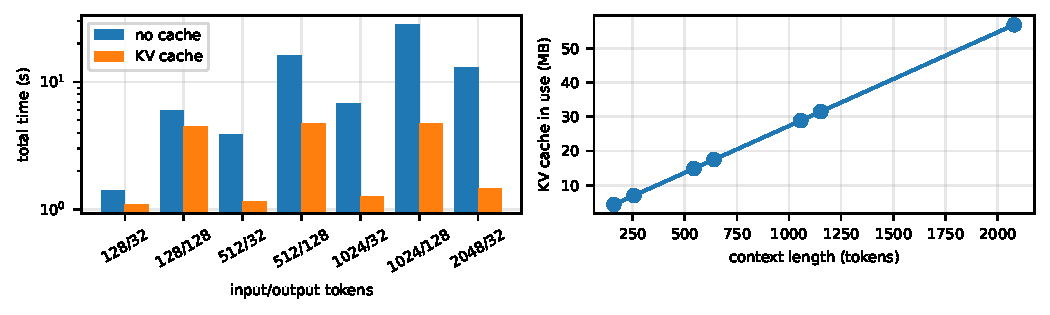
\includegraphics[width=\columnwidth]{fig_cache.pdf}
\caption{Left: total generation time with and without the KV cache. Right: KV cache bytes in use versus context length.}
\label{fig:cache}
\end{figure}

\subsection{Tiled Attention with Online Softmax (Task 4)}\label{sec:attn}
We tested 64 cases (8 shapes with batch 1--2, 4--14 heads, $T_q\in\{1,5,16,33,100,128,257,512\}$ and $T_k\ge T_q$, causal and non-causal, query scales 1 and 8 to stress the softmax, fp32 and fp16; tile sizes 32 and 128) against an fp64 reference. Table~\ref{tab:attnnum} shows that in fp32 the maximum absolute error of the tiled kernel ($1.6\times10^{-5}$) is comparable to that of the dense reference ($1.5\times10^{-5}$) and of PyTorch's SDPA ($1.4\times10^{-5}$), and that the tiled output differs from the dense reference by at most $8.4\times10^{-6}$; in fp16 all implementations are dominated by output rounding ($1.9\times10^{-3}$). The tiled kernel also drives the full model: greedy generation with it is token-identical to the SDPA path on the four prompts tested (24 tokens each).

\begin{table}[t]
\caption{Error versus an fp64 reference over all test shapes (max and mean absolute error).}
\label{tab:attnnum}
\centering\scriptsize
\begin{tabular}{lcccc}\toprule dtype & ref & tiled & tiled(128) & SDPA\\\midrule
float32 max err & 1.5e-05 & 1.6e-05 & 1.5e-05 & 1.4e-05\\
float32 mean err & 1.6e-07 & 1.6e-07 & 1.6e-07 & 2.0e-07\\
float16 max err & 1.9e-03 & 1.9e-03 & 1.9e-03 & 1.9e-03\\
float16 mean err & 6.9e-05 & 6.9e-05 & 6.9e-05 & 7.6e-05\\
\bottomrule\end{tabular}
\end{table}

Table~\ref{tab:attnperf} and Fig.~\ref{fig:attn} compare speed and memory (fp16, 12 heads, $d{=}128$, causal prefill). The tiled kernel needs far less memory than the dense reference---51\,MB versus 2,316\,MB at $T{=}4096$, a factor of 45, and growing linearly rather than quadratically---but it is 5 times \emph{slower} than the dense reference and 120 times slower than PyTorch's fused SDPA (374.9\,ms versus 71.6\,ms and 3.06\,ms). This is expected: our tiles are separate PyTorch kernel launches with intermediate tensors written to GPU memory, while fused kernels keep tiles in on-chip memory. The educational implementation therefore demonstrates the algorithm and its memory behaviour, not a speed advantage.

\begin{table}[t]
\caption{Attention speed and peak extra memory (fp16, 12 heads, $d{=}128$, causal).}
\label{tab:attnperf}
\centering\scriptsize
\begin{tabular}{rrrrrrr}\toprule T & ref ms & tiled ms & SDPA ms & ref MB & tiled MB & SDPA MB\\\midrule
256 & 0.62 & 2.07 & 0.11 & 10 & 8 & 2\\
512 & 1.68 & 6.17 & 0.27 & 38 & 10 & 3\\
1024 & 5.70 & 22.39 & 0.45 & 148 & 15 & 7\\
2048 & 17.38 & 74.08 & 0.88 & 582 & 27 & 12\\
4096 & 71.61 & 374.85 & 3.06 & 2316 & 51 & 24\\
\bottomrule\end{tabular}
\end{table}

\begin{figure}[t]
\centering
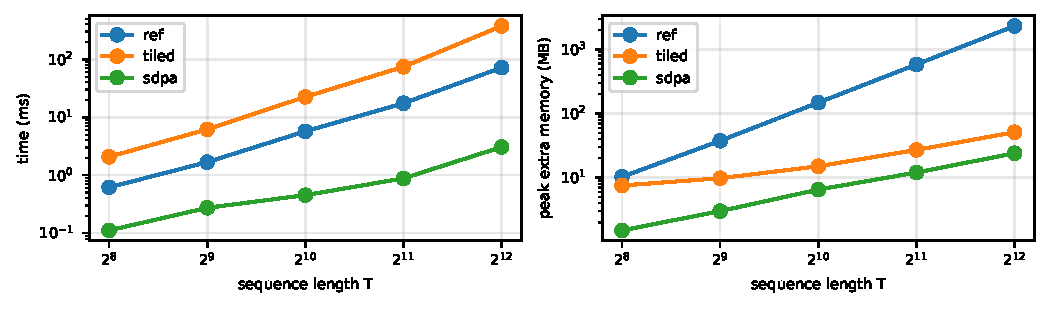
\includegraphics[width=\columnwidth]{fig_attn.pdf}
\caption{Attention time (left) and peak extra memory (right) versus sequence length.}
\label{fig:attn}
\end{figure}

\subsection{Speculative Decoding (Task 5)}
The draft is the fine-tuned Qwen2.5-0.5B (same tokenizer; 0.92\,GB in fp16; 12\,KiB KV cache per token), the target the fine-tuned 1.5B model; we run the 40 test prompts $\{0,5,10,\dots\}$ with the natural stop token. Table~\ref{tab:spec} and Fig.~\ref{fig:spec} give the results. Acceptance is high (94\% for $K{=}2$, 86--87\% for $K{\ge}4$) because the answer is a short, nearly deterministic JSON string, and a round emits 2.8--5.5 tokens. In fp16, 38 of 40 outputs are token-identical to target-only greedy decoding for every $K$; the two mismatches (prompts 5 and 90, at generated positions 4 and 11) are the same for all $K$. In fp32 the decoder is identical on all 20 prompts tested, so the two fp16 mismatches come from the target's $(K{+}1)$-token verification pass having different rounding from the one-token pass, which flips a near-tie; they do not indicate a logic error. Hugging Face assisted generation (with the penalty disabled) agrees with our cached greedy output on 18 of 20 prompts, the same kind of fp16 differences.

Despite the high acceptance, speculative decoding is \emph{slower} than plain cached decoding: $0.90\times$, $0.82\times$ and $0.81\times$ for $K{=}2,4,6$. The measurements explain why. In an isolated, synchronised measurement at a 512-token context the 0.5B draft takes 43.07\,ms per decoded token and the 1.5B target 43.03\,ms (cost ratio $c{=}1.00$; the pipelined decode loop of Table~\ref{tab:cache} is somewhat faster, about 35\,ms per token), because both are limited by launch overhead of 24 vs.\ 28 layers rather than by arithmetic; a 5-token verification pass costs 39\,ms, as much as a single-token step. A round with $K$ drafts therefore costs about $K\cdot 43+39$\,ms and emits $\bar n$ tokens, giving $\approx\bar n/(K+0.9)$ times the cached speed: $2.80/2.9{=}0.97$ for $K{=}2$ and $4.19/4.9{=}0.86$ for $K{=}4$, close to the measured values (the remainder is synchronisation of host-side comparisons). A speedup would require a cheaper draft step, e.g.\ via CUDA graphs or a fused decoder (for $c{=}0.3$, $K{=}4$ the same model predicts $4.19/(4\cdot0.3+0.9)\approx2.0\times$; this projection is not measured). Peak extra memory for speculative decoding is only 26--27\,MB beyond the resident weights of both models (about 4.0\,GB).

\begin{table}[t]
\caption{Greedy speculative decoding on 40 real test prompts (fp16). Latency is per prompt; speedup is cached time divided by speculative time.}
\label{tab:spec}
\centering\scriptsize
\begin{tabular}{rcccccc}\toprule K & Token-identical & Accept. & Tok/round & Spec s & Cached s & Speedup\\\midrule
2 & 38/40 & 0.94 & 2.80 & 0.650 & 0.584 & 0.90$\times$\\
4 & 38/40 & 0.87 & 4.19 & 0.686 & 0.560 & 0.82$\times$\\
6 & 38/40 & 0.86 & 5.53 & 0.697 & 0.562 & 0.81$\times$\\
\bottomrule\end{tabular}
\end{table}

\begin{figure}[t]
\centering
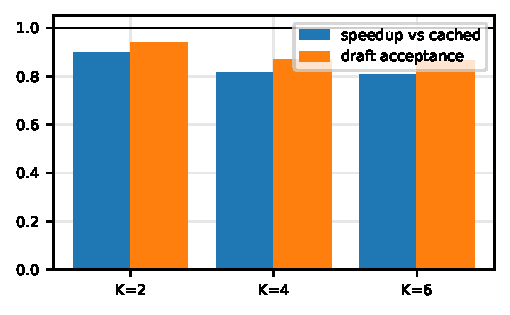
\includegraphics[width=0.8\columnwidth]{fig_spec.pdf}
\caption{Speculative decoding: speedup relative to cached decoding (values below 1 are slowdowns) and draft acceptance rate for each $K$.}
\label{fig:spec}
\end{figure}

\subsection{Application (Task 6)}
The browser application (FastAPI back end, single-page front end, no notebook needed) loads both models once at start-up, shows loading progress and the device, and offers five tabs. \emph{Screening} accepts a pasted note and any number of criteria, runs the chosen decoder, and for each criterion shows the label, the cited sentences with their text, an evidence-based explanation, flags (\emph{unsupported}, invalid output, non-existent sentence IDs), timing and, for speculative mode, the draft acceptance; it aggregates the labels with rules R1--R4 and exports an HTML or JSON report containing provenance (models, adapter checksum, mode, timestamp) and the research-prototype disclaimer. \emph{Inference lab} runs the same criteria through the three decoders, reporting time, tokens/s, peak GPU memory, draft acceptance and a token-equality check. \emph{Attention lab} runs the reference, tiled and SDPA kernels on random tensors of the requested size and reports time, memory and error against fp64. \emph{Experiments} renders the saved result tables. Invalid inputs (empty or oversize note, malformed criteria, unknown mode, out-of-range attention parameters) return readable error messages and leave the server running. We exercised the HTTP interface with a synthetic note and five criteria in the cached and speculative modes (identical labels and evidence), the comparison and attention endpoints (all three decoders token-identical), and each error case. On the synthetic case the application flagged two exclusion answers (``heart failure'', ``anticoagulant therapy'') as unsupported because the model labelled them \emph{not excluded} without citing evidence, even though the note states that the patient denies heart failure: an example of the exclusion weakness discussed above and of why such flags are shown to the user.
